\documentclass[20pt]{article}

\usepackage[a4paper]{geometry}
\usepackage{titlesec}
\usepackage{amsmath}
\usepackage{amssymb}
\usepackage{times}
\usepackage{tipa}
\usepackage{covington}
\usepackage{tikz-qtree}

\setlength\parindent{0pt}
\newcommand{\ipa}[1]{\textipa{#1}}
\newcommand{\broad}[1]{/\ipa{#1}/}
\newcommand{\narrow}[1]{[ \ipa{#1} ]}
\newcommand{\english}[1]{$<$#1$>$}
\newcommand{\sk}[0]{{\kern 0.05em}}
\newcommand{\mk}[0]{{\kern 0.1em}}
\newcommand{\smallcapi}[0]{\sk\textsci\sk}
\newcommand{\openo}[0]{\sk O}

\titlespacing*{\section}{0pt}{0.7\baselineskip}{0.7\baselineskip}
\titleformat*{\section}{\large\bfseries}

\begin{document}

\Large\textbf{Problem Set 2} \\
\normalsize
Alice McKean \\
\today


\section{Lexical Categories}
Clean is a verb as it can reflect tense information: ``Jane cleaned our plates.''

Clean is an adjective as it can be prefixed by ``un+'':
``The unclean toilet stank.'' \\

\par

Sound is a noun as it can be pluralized: ``Jacob heard many spooky sounds.''

Sound is a verb as it can reflect tense information: ``You sounded scared last night.''

Sound is an adjective as it can be prefixed by ``un+'': ``The unsound plan
required Joan.'' \\


Back is a noun as it can be pluralized: ``He scratched our backs.''

Back is a verb as it can reflect tense information:
``She backed into the corner.'' \\


Can is an auxiliary as it can invert: ``You can speak Russian.'' and
``Can you speak Russian?''.

Can is a noun as it can be pluralized: ``Jim opened three cans.''

Can is a verb as it can reflect tense information: ``She was canning the fish.''

\section{Acceptability Judgments}  

My analysis:
\begin{enumerate}
  \itemsep0em 
  \item[5a] Grammatical
  \item[5b] Pragmatically anomalous. This is a semantically well formed sentence as
    every tall person will be tall before a party starts. It is pragmatically
    anomalous as people do not normally change height during the course of a
    party.
  \item[6a] Grammatical
  \item[6b] Ungrammatical as there is no way to parse the conjunction into a
    parse tree that matches the intended interpretation.
  \item[7]  Ungrammatical them* requires number agreement with the referent.
  \item[8a] Grammatical
  \item[8b] Ungrammatical gathered requires number agreement with the referent.
\end{enumerate}


Consultant 1:
\begin{enumerate}
  \itemsep0em 
  \item[5a] Fine
  \item[5b] That doesn't make sense. Why would she get any taller?
  \item[6a] Fine
  \item[6b] That doesn't make sense.
  \item[7]  It should be them instead.
  \item[8a] Fine
  \item[8b] Fine
\end{enumerate}

\newpage

Consultant 2:
\begin{enumerate}
  \itemsep0em 
\item[5a] Fine
\item[5b] That sounds weird. Tall is something that you are.
\item[6a] Fine
\item[6b] That sounds weird. It is asking a question and a statement at the
  same time.
\item[7]  That is wrong. You should use them.
\item[8a] Fine
\item[8b] One protester couldn't gather. Who would you be gathering with?
\end{enumerate}

Consultant 3:
\begin{enumerate}
  \itemsep0em 
  \item[5a] Fine
  \item[5b] That makes grammatical sense but doesn't make semantic sense.
  \item[6a] Fine
  \item[6b] That doesn't make grammatical sense. It is a question and a part
    added on as if it is a declarative sentence.
  \item[7]  Themselves seems like it should be them in this context because
    you're the one telling the story not the children.
  \item[8a] Fine
  \item[8b] Sounds wrong. Only a group of something can gather.
\end{enumerate}

Interestingly Consultant 1 thought that sentence 8b was fine. In order to not
introduce bias I only read the sentence once unless I was asked to read it
again. It could have just been that they didn't notice that protesters was not
pluralized.

\newpage

\section{Tree Drawing}

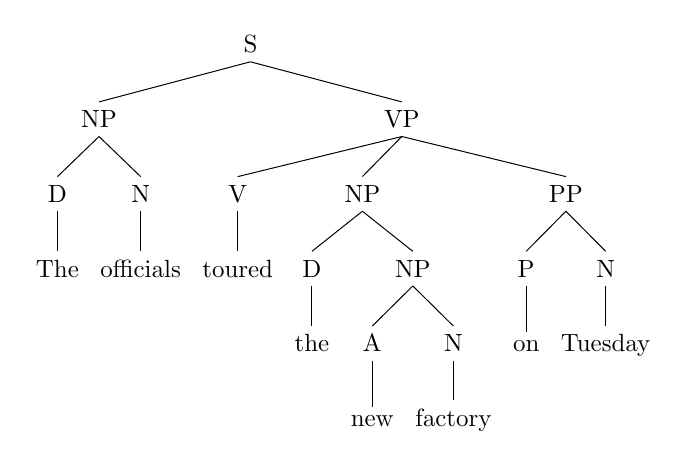
\begin{tikzpicture}[scale=0.9, transform shape]
  \Tree [.S [.NP [.D The ]
                 [.N officials ]
            ]
            [.VP [.V toured ]
                 [.NP [.D the ]
                      [.NP [.A new ]
                           [.N factory ]
                      ]
                 ]
                 [.PP [.P on ]
                      [.N Tuesday ]
                 ]
            ]
        ]
\end{tikzpicture}

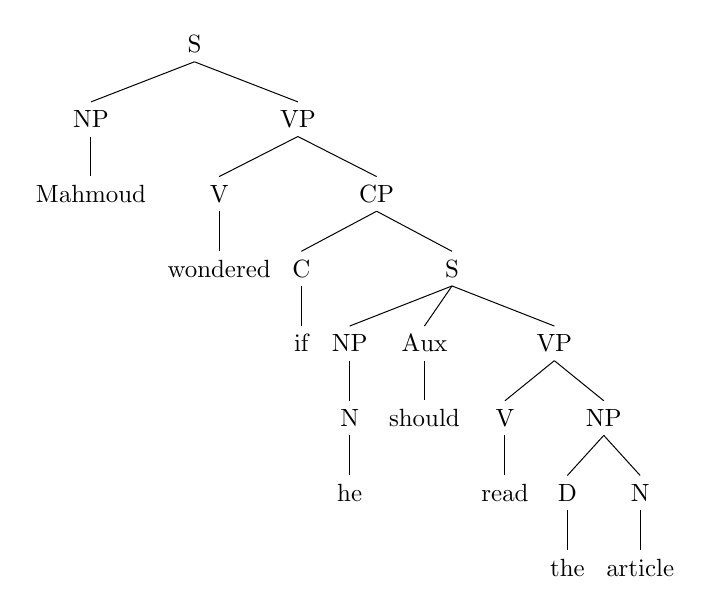
\begin{tikzpicture}[scale=0.9, transform shape]
  \Tree [.S [.NP Mahmoud ]
            [.VP [.V wondered ]
                 [.CP [.C if ]
                      [.S [.NP [.N he ] ]
                          [.Aux should ]
                          [.VP [.V read ]
                               [.NP [.D the ]
                                    [.N article ]
                               ]
                          ]
                      ]
                 ]
            ]
        ]
\end{tikzpicture}

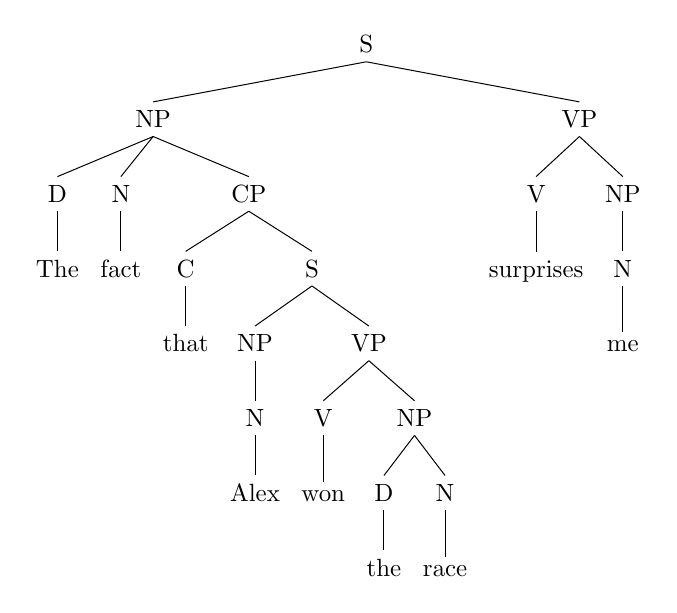
\begin{tikzpicture}[scale=0.9, transform shape]
  \Tree [.S [.NP [.D The ]
                 [.N fact ]
                 [.CP [.C that ]
                      [.S [.NP [.N Alex ]]
                          [.VP [.V won ]
                               [.NP [.D the ]
                                    [.N race ]
                               ]
                          ]
                      ]
                 ]
            ]
            [.VP [.V surprises ]
                 [.NP [.N me ]]
            ]
        ]
\end{tikzpicture}

\end{document}

